\documentclass[tikz,border=3pt]{standalone}
\usepackage[utf8]{inputenc}
\usepackage[T1]{fontenc}
\usepackage{lmodern}
\renewcommand{\familydefault}{\sfdefault}
\usepackage{sansmath}\sansmath
\usepackage{chemfig}
\usepackage{pgfplots}\pgfplotsset{compat=1.18,/pgf/number format/use comma,/pgf/number format/1000 sep={.}}
\usetikzlibrary{arrows.meta,calc,positioning,decorations.pathmorphing,patterns}
% paleta del sitio
\definecolor{nar}{HTML}{E8680C}\definecolor{narc}{HTML}{FFB35C}\definecolor{hielo}{HTML}{FFF3E8}
\definecolor{tinta}{HTML}{1D1D1F}\definecolor{gris}{HTML}{6E6E73}\definecolor{lila}{HTML}{7C5CF0}
\definecolor{azul}{HTML}{2F6FD6}\definecolor{menta}{HTML}{17A673}\definecolor{coral}{HTML}{E8342A}
\begin{document}
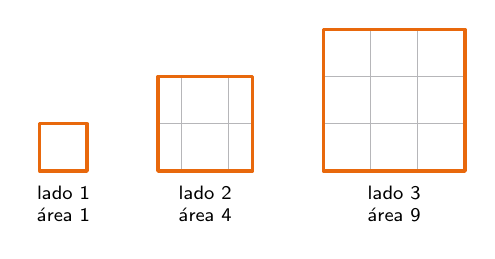
\begin{tikzpicture}[font=\small,x=0.6cm,y=0.6cm,line cap=round,line join=round,step={(1,1)}]
\draw[gris!50] (0,0) grid (1,1); \draw[nar,very thick] (0,0) rectangle (1,1);
\draw[gris!50] (2.5,0) grid (4.5,2); \draw[nar,very thick] (2.5,0) rectangle (4.5,2);
\draw[gris!50] (6,0) grid (9,3); \draw[nar,very thick] (6,0) rectangle (9,3);
\node[below,font=\scriptsize,align=center] at (0.5,-0.1) {lado 1\\área 1};
\node[below,font=\scriptsize,align=center] at (3.5,-0.1) {lado 2\\área 4};
\node[below,font=\scriptsize,align=center] at (7.5,-0.1) {lado 3\\área 9};
\end{tikzpicture}
\end{document}
